\documentclass{article}
\usepackage{times}
\usepackage[T1]{fontenc}
\usepackage[portuges]{babel}


% Comentar para not MAC Users
\usepackage[utf8]{inputenc}

\usepackage{a4}
%\usepackage[margin=3cm,nohead]{geometry}
\usepackage{textgreek}
\usepackage{epstopdf}
\usepackage{graphicx}
\usepackage{fancyvrb}
\usepackage{amsmath}
\usepackage{float}
\usepackage{listings}
%\renewcommand{\baselinestretch}{1.5}



\begin{document}
\title{Computação Gráfica}
\author{Etienne Costa(A76089) \and Joana Cruz(A76270) \and Rafael Alves(A72629) \and Maurício Salgado(por numero)}
\date{}
\maketitle
\newpage
\section{Introdução}
O relátorio apresentado diz respeito à primeira fase do trabalho proposto no âmbito da unidade curricular de Computação Gráfica. O trabalho
consiste no desenvolvimento de um gerador de vértices de algumas primitivas gráficas(plano, caixa, esfera e cone). Para além disto, também foi desenvolvida
uma aplicação de leitura de ficheiros de configuração em XML que servirá para desenhar os vértices anteriormente gerados.
\newpage
\section{Generator}
A função main do gerador vê qual a primitiva gráfica que se pretende gerar, como já referimos, pode ser um plano, uma caixa, uma esfera ou um cone.
De seguida chama a função geradora correspondente, tendo em conta o número de argumentos pedidos, e escreve como resultado os vértices gerados.\newline
\begin{itemize}
\item\textbf{Plano} - apenas recebe um argumento, por ser pedido um plano quadrado e corresponde ao lado do plano. 
\item\textbf{Caixa} - recebe como argumentos o comprimento, a altura, a largura e o número de divisões. Caso não se pretenda dividir esse argumento tomará o valor 1.
\item\textbf{Esfera} - recebe como argumentos o raio, o número de slices(divisões verticais) e o número de stacks(divisões horizontais).
\item\textbf{Cone} -
\end{itemize}
\newpage
\section{Plano}
É pretendido um plano $XZ$ quadrado, centrado na origem e feito com 2 triângulos. 
Para calcular os pontos que constituem o plano precisamos do tamanho de cada lado que nos dará informação sobre a dimensão do plano
no eixo dos $xx$, e dimensão do plano no eixo dos $zz$. 
O plano contém 4 pontos e sendo centrado na origem temos que efetuar os seguintes cálculos: \newline
\begin{center}
$x = tamanho/2$ \newline
$y = 0$ \newline
$z = tamanho/2$ \newline
\end{center}
\begin{figure}[H]
\centering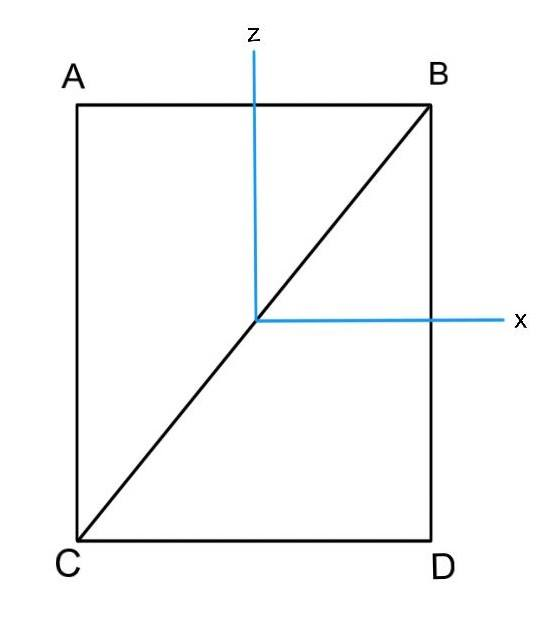
\includegraphics[scale=0.35]{plano} 
\caption{\label{fig:controller}Figura ilustrativa de um plano XZ}
\end{figure} 
Efetuando os cálculos, obtemos os seguintes pontos: \newline
\begin{center}
$A = (-x,0,z)$ \newline 
$B = (x,0,z)$ \newline 
$C = (-x,0,-z)$ \newline 
$D = (x,0,-z)$ \newline
\end{center}
Pelo que obtemos as seguintes coordenadas para os vértices dos triângulos $ABC$ e $BCD$, terão como coordenadas: \newline
\begin{center}
$ABC\rightarrow (-x,y,z) (x,y,z) (-x,y,-z)$ \newline
$BCD\rightarrow (x,y,z) (-x,y,-z) (x,y,-z)$ \newline
\end{center}
Caso fosse pedido qualquer plano $XZ$ teríamos que receber dois parâmetros: as dimensões do plano no eixo do xx e no eixo zz. 
\newpage
\section{Caixa}
Para obtermos uma caixa necessitamos dos seguintes parametros compromento(dimensao do X), altura(dimensao do Y), largura(dimensao do Z) e o número de divisoes. 
Uma caixa pode conter divisoes ou não, por esse motivo precisamos de guardar as dimensoes de cada divisao. 
Precisamos de calcular as faces XY, as faces XZ e as faces YX 
\newpage
\section{Esfera}
O cálculo dos pontos de uma esfera necessita de 3 parâmetros: raio, slices que correspondem às divisoes na vertical ao longo da esfera e stacks que correspondem às divisoes na horizontal ao longo da esfera
Quanto maior o número de slices e stacks, maior será o número de pontos a determinar, ou seja, melhor será a precisão da esfera. Sabemos que:
\begin{itemize}
\item A intersecção entre uma slice e uma stack origina 4 pontos
\item A distância entre cada um destes pontos ao centro é o raio
\item Podemos ter um vetor para cada ponto, e esse vetor tem dois ângulos, um relativo ao eixo dos $yy$(\textbeta) e outro relativo ao eixo dos $zz$(\textalpha). Em vez de termos relativo ao eixo dos zz, poderíamos ter relativo ao eixo dos xx
\item O ângulo \textalpha $\in$ [0; 2$\pi$] e depende do número de slices
\item O ângulo \textbeta $\in$ [0; $\pi$], e depende do número de stacks
\item Temos um \textDelta\textalpha \ que será calculado através $\frac{2\times\pi}{slices}$
\item Temos um \textDelta\textbeta \ que será calculado através $\frac{\pi}{stacks}$
\end{itemize}
\begin{figure}[H]
\centering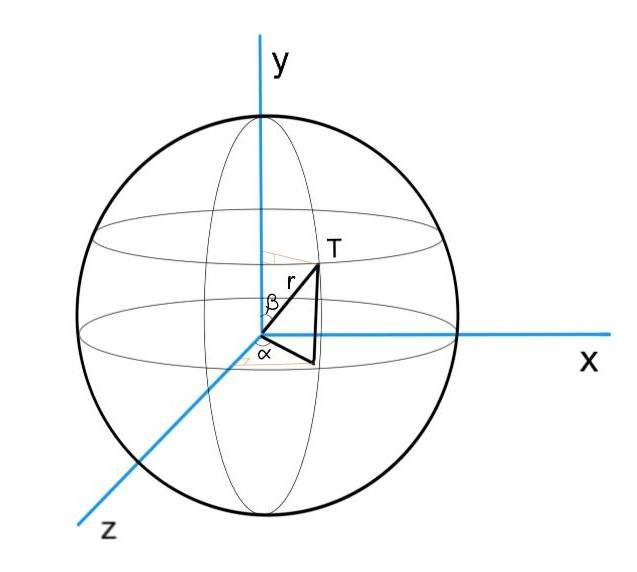
\includegraphics[scale=0.50]{esfera} 
\caption{\label{fig:controller}Representação de um ponto T na superfície de uma esfera e os respetivos ângulos}
\end{figure}
Após a nossa representação da esfera, facilmente conseguimos retirar as equações para obter as coordenadas do ponto T:
\begin{center}
$x = r \times \sin(b) \times \sin(a)$

$y = r \times \cos(b)$

$z = r \times \sin(b) \times \cos(a)$ 
\end{center}
\begin{figure}[H]
\centering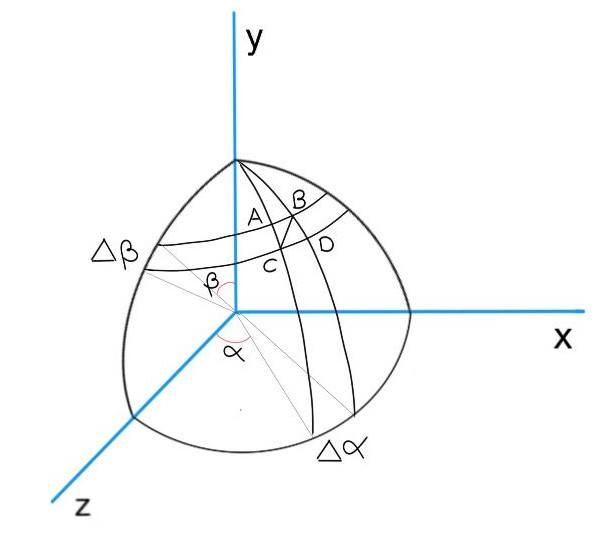
\includegraphics[scale=0.50]{esfera1} 
\caption{\label{fig:controller}Representação dos 4 pontos de uma interseção}
\end{figure}
Na figura acima apresentada demonstramos um exemplo de uma interseção entre slices e stacks em que geramos os pontos $A,B,C$ e $D$.
Estes pontos servirão para calcular os vértices correspondentes aos triângulos $ABC$ e $BCD$. Por último falta-nos determinar, os ângulos correspondentes
aos pontos $B, C$ e $D$.\newline
\begin{center}
\begin{tabular}{||c c c||} 
\hline
Ponto & \textalpha & \textbeta \\ [0.5ex] 
\hline\hline
B & \textalpha + \textDelta\textalpha & \textbeta\\ 
\hline
C & \textalpha & \textbeta + \textDelta\textbeta \\
\hline
D & \textalpha + \textDelta\textalpha & \textbeta + \textDelta\textbeta\\ [1ex] 
    \hline
\end{tabular}
\end{center}
Para cada stack i $\{$\newline
\par $\beta = i \times \Delta\beta$ \newline
\par Para cada slice j $\{$ \newline
\par $\alpha = j \times \Delta\alpha$ \newline\newline
\par\textit{Ponto A} \newline
\par$x = r\times\sin(\beta)\times\sin(\alpha)$ \newline
\par$y = r\times\cos(\beta)$ \newline
\par$z = r\times\sin(\beta)\times\cos(\alpha)$ \newline\newline
\par\textit{Ponto B} \newline
\par$x = r\times\sin(\beta)\times\sin(\alpha + \Delta\alpha)$ \newline
\par$y = r\times\cos(\beta)$ \newline
\par$z = r\times\sin(\beta)\times\cos(\alpha + \Delta\alpha)$ \newline\newline
\par\textit{Ponto C} \newline
\par$x = r\times\sin(\beta + \Delta\beta)\times\sin(\alpha + \Delta\alpha)$ \newline
\par$y = r\times\cos(\beta + \Delta\beta)$ \newline
\par$z = r\times\sin(\beta + \Delta\beta)\times\cos(\alpha + \Delta\alpha)$ \newline\newline
\par\textit{Ponto D} \newline
\par$x = r\times\sin(\beta + \Delta\beta)\times\sin(\alpha)$ \newline
\par$y = r\times\cos(\beta + \Delta\beta)$ \newline
\par$z = r\times\sin(\beta + \Delta\beta)\times\cos(\alpha)$ \newline
\par $\}$ \newline
$\}$ 
\newpage
\section{Cone}
\newpage
\section{Conclusão}
\end{document}